\chapter{$^{57}$Co spectra measurement with integrated amplifier} 

To properly test the assembled PCB with attached S14605 photodiode (further referred as Si PIN detector) and to compare its detection efficiency for 14.4 keV photons with the detection efficiency of the other types of detectors - scintillator and gaseous detectors, the measurement setup with carefully designed geometry was constructed.

%\par
%
%The goal is to compare the Si PIN detector's detection efficiency of 14.4 keV photons with the detection efficiency of the other detectors - the scintillator and gaseous detectors.

\par

The onboard amplification is set in a way to have 14.4 keV energy peak in the second half of the channel range, which on the other hand result into the saturation of the higher energies, but the detection of these energies is not our focus.



\section{Measurement setup}
The measurement setup mainly consist of 3D printed parts - plastic holders for every detector and holders for radiation filters. All the holders have to be modular and easily interchangeable to allow the geometry to be kept same for every detector.
$^{57}$Co 2020 source is mounted onto the transducer (switched off in this measurement). Due to the fact, that the detectors have a different size of detection area, the irradiation has to be done through a collimator. To compare detection efficiency of the defined detection surface, the detector is irradiated through a hole ($d = 4$ mm) in a lead shielding, which works as collimator for $^{57}$Co source.

\par
For every detector, the sequence of five measurement was performed - without filter, with three filters and without a source. The relative detection efficiency for 14.4 keV is determined by Gaussian fit of the 14.4 keV peak in spectra with subtracted background. Every measurement of spectra ran 1200 s of live time.


\begin{figure}[H]
 \centering
 
\includegraphics[scale=0.8, angle = 90]{./pictures/NoPicture.jpg}
 \caption{Measurement setup.}
 \label{meas setup}
 
\end{figure}

\section{Si PIN detector measurement}

The output SMA connector is connected directly to the ORTEC MCA.
Three filters were placed before lead collimator - Cu (255 $\mu$m), Al (780 $\mu$m), Pb (5 mm).

\begin{figure}[H]
 \centering
 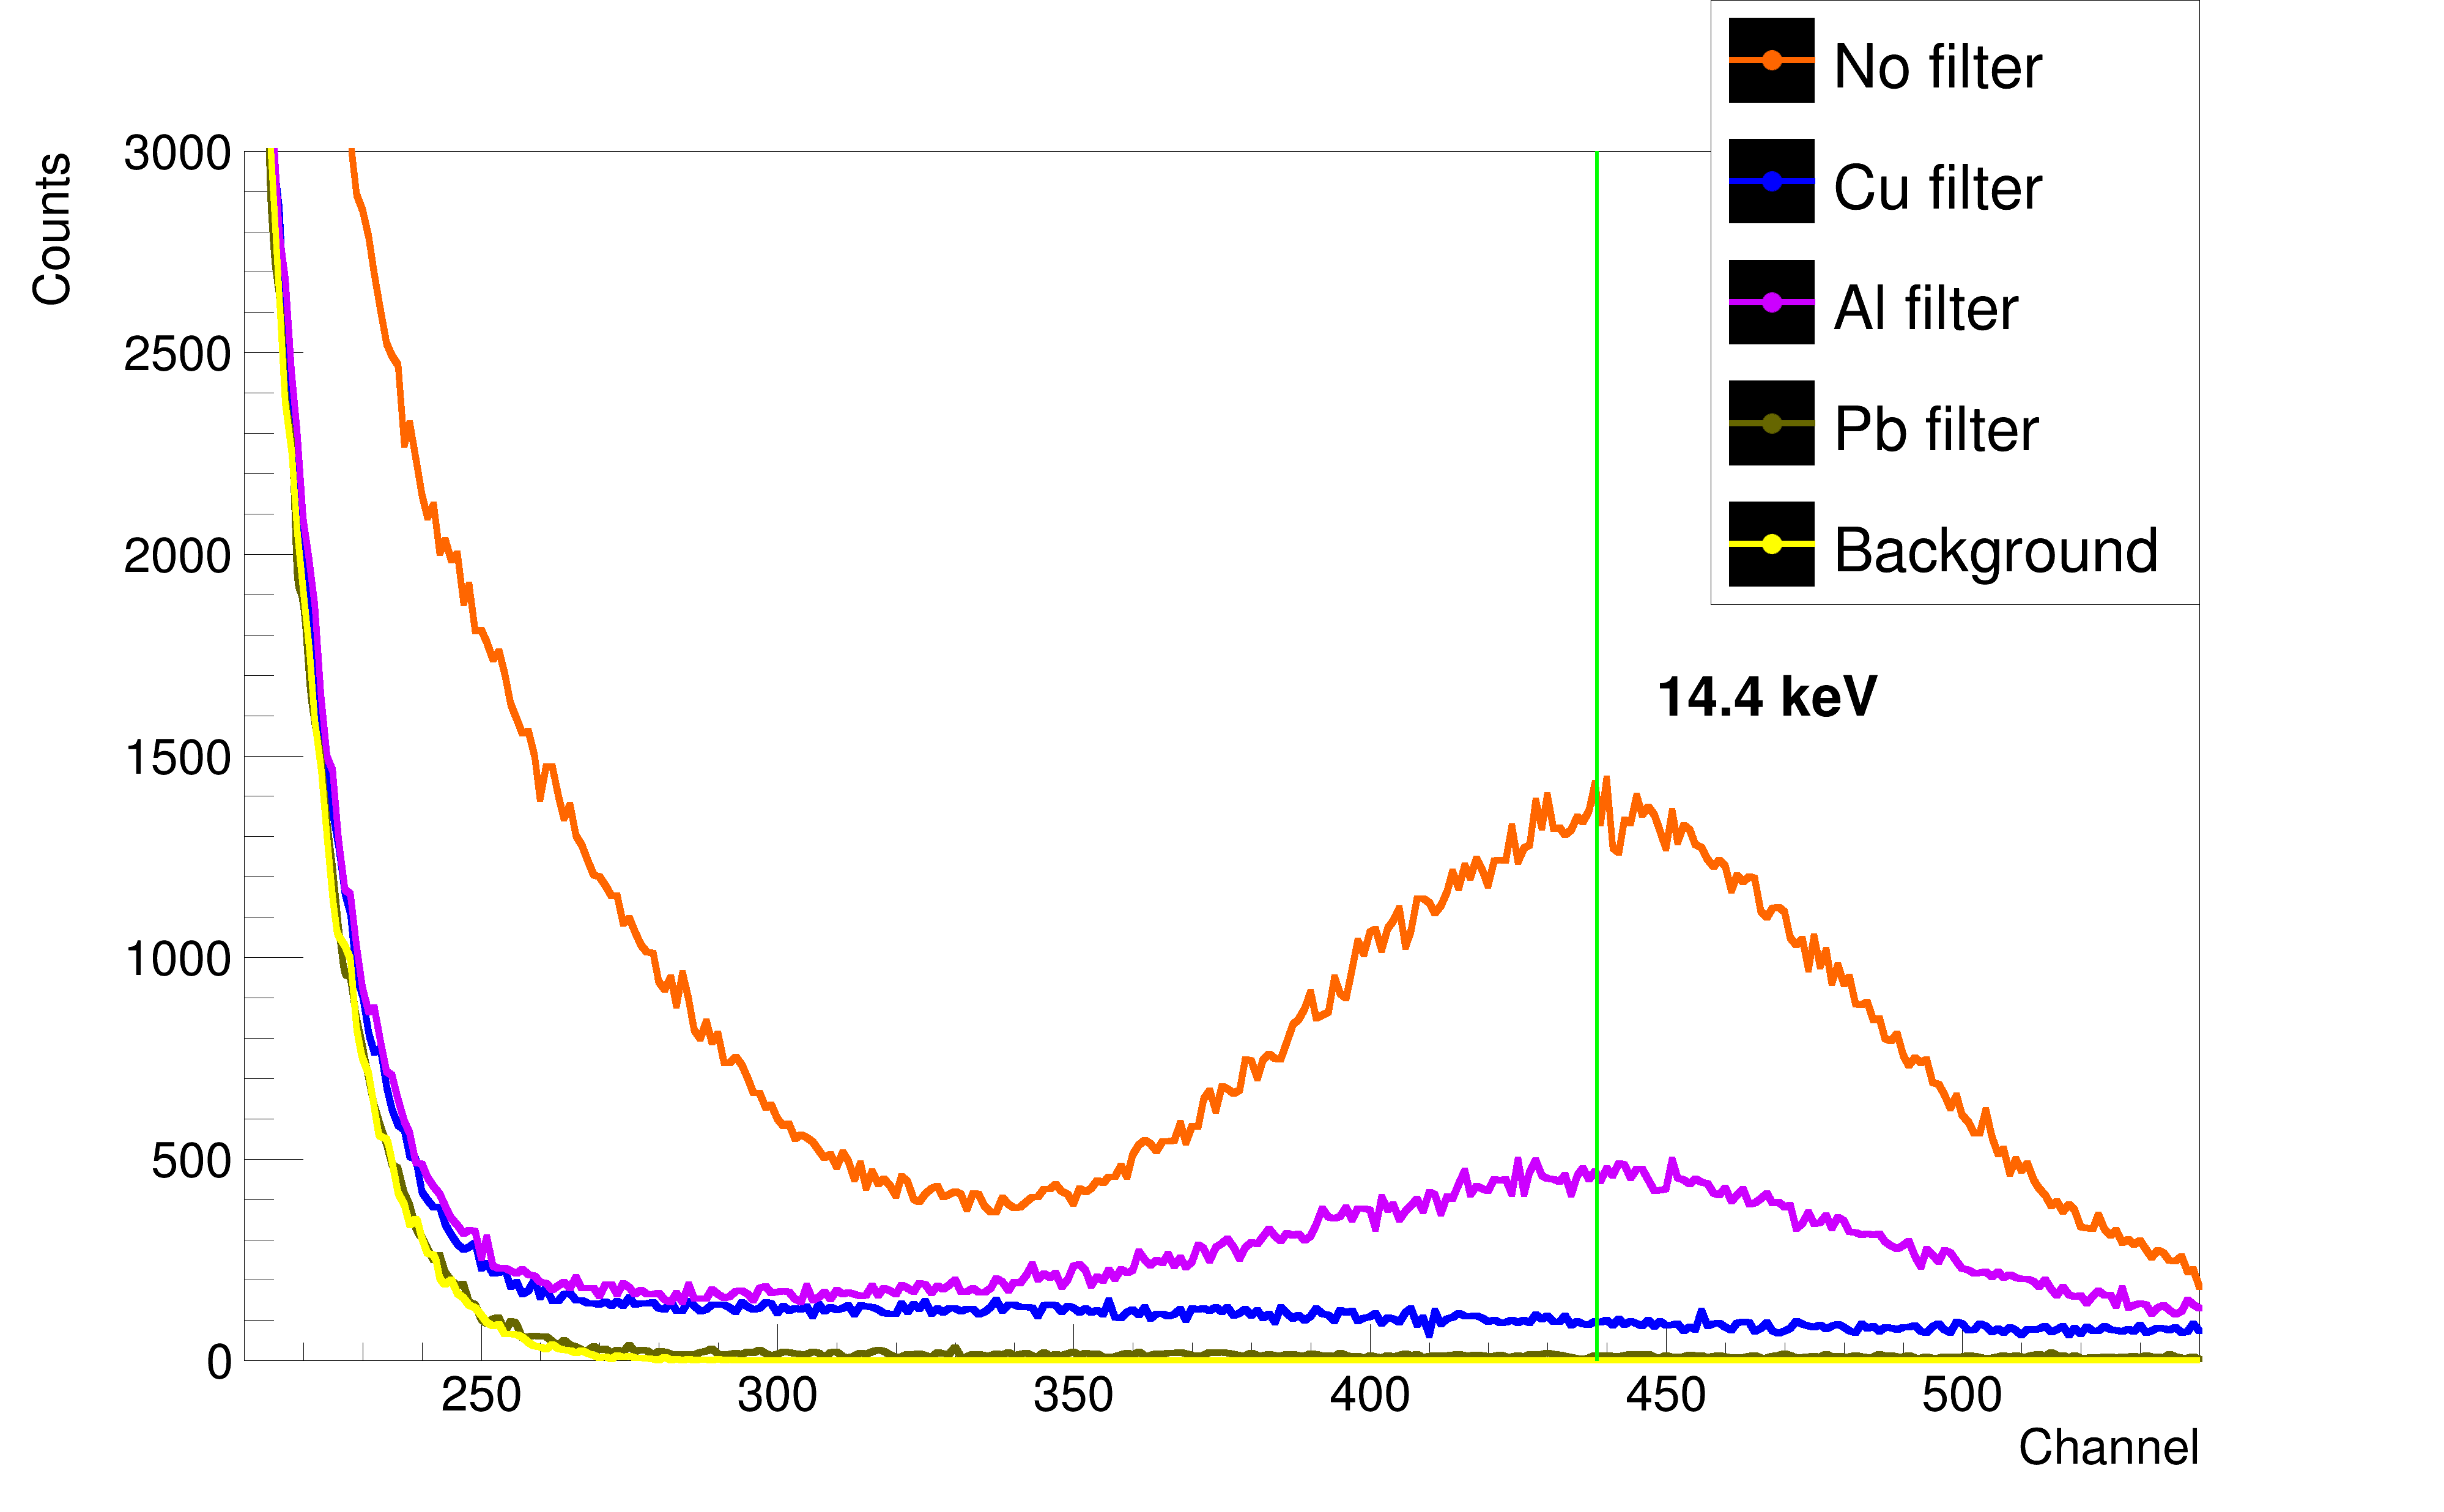
\includegraphics[scale=0.125, angle = 0]{./pictures/SemiSpectre.png}
 \caption{Si PIN detector $^{57}$Co spectra.}
 \label{Si PIN detector spectra.}
\end{figure}


It can be seen, that the noise in spectrum is much lesser than in case of ORTEC setups. The part of 6.4 keV peak can be also seen. Various ways were performed in order to reduce noise - cooling by ice, improving the shielding etc. However, none of them resulted into 6.4 keV energy peak without noise. Main part of remaining noise probably arises from Si PIN diode capacity ($C_{\textrm{S14605}} \approx 25$ pF). This fact can be confirmed by using the same PCB with photodiode with smaller capacity (for example BPW34, $C_{\textrm{BPW34}} \approx 10$ pF). Spectra of BPW34 attached to PCB can be seen in the Fig.



\section{Scintillator and gaseous detector measurement}
To measure the scintillator and the gaseous detector relative efficiency the same setup was used. As a gaseous detector was used tube LND45479, optimized for the 14.4 keV detection with amplification electronics based also on Cremat modules. In case of scintillator detector, our choice was photomultiplier tube R6095 \cite{R6095} with C9028-01 socket \cite{C9028}. As a scintillator crystal was used 0.4 mm thick YAP(Ce) and the amplification is done by the custom made amplifier\cite{STEJSKAL2019thesis}.

\begin{figure}[H]
\centering
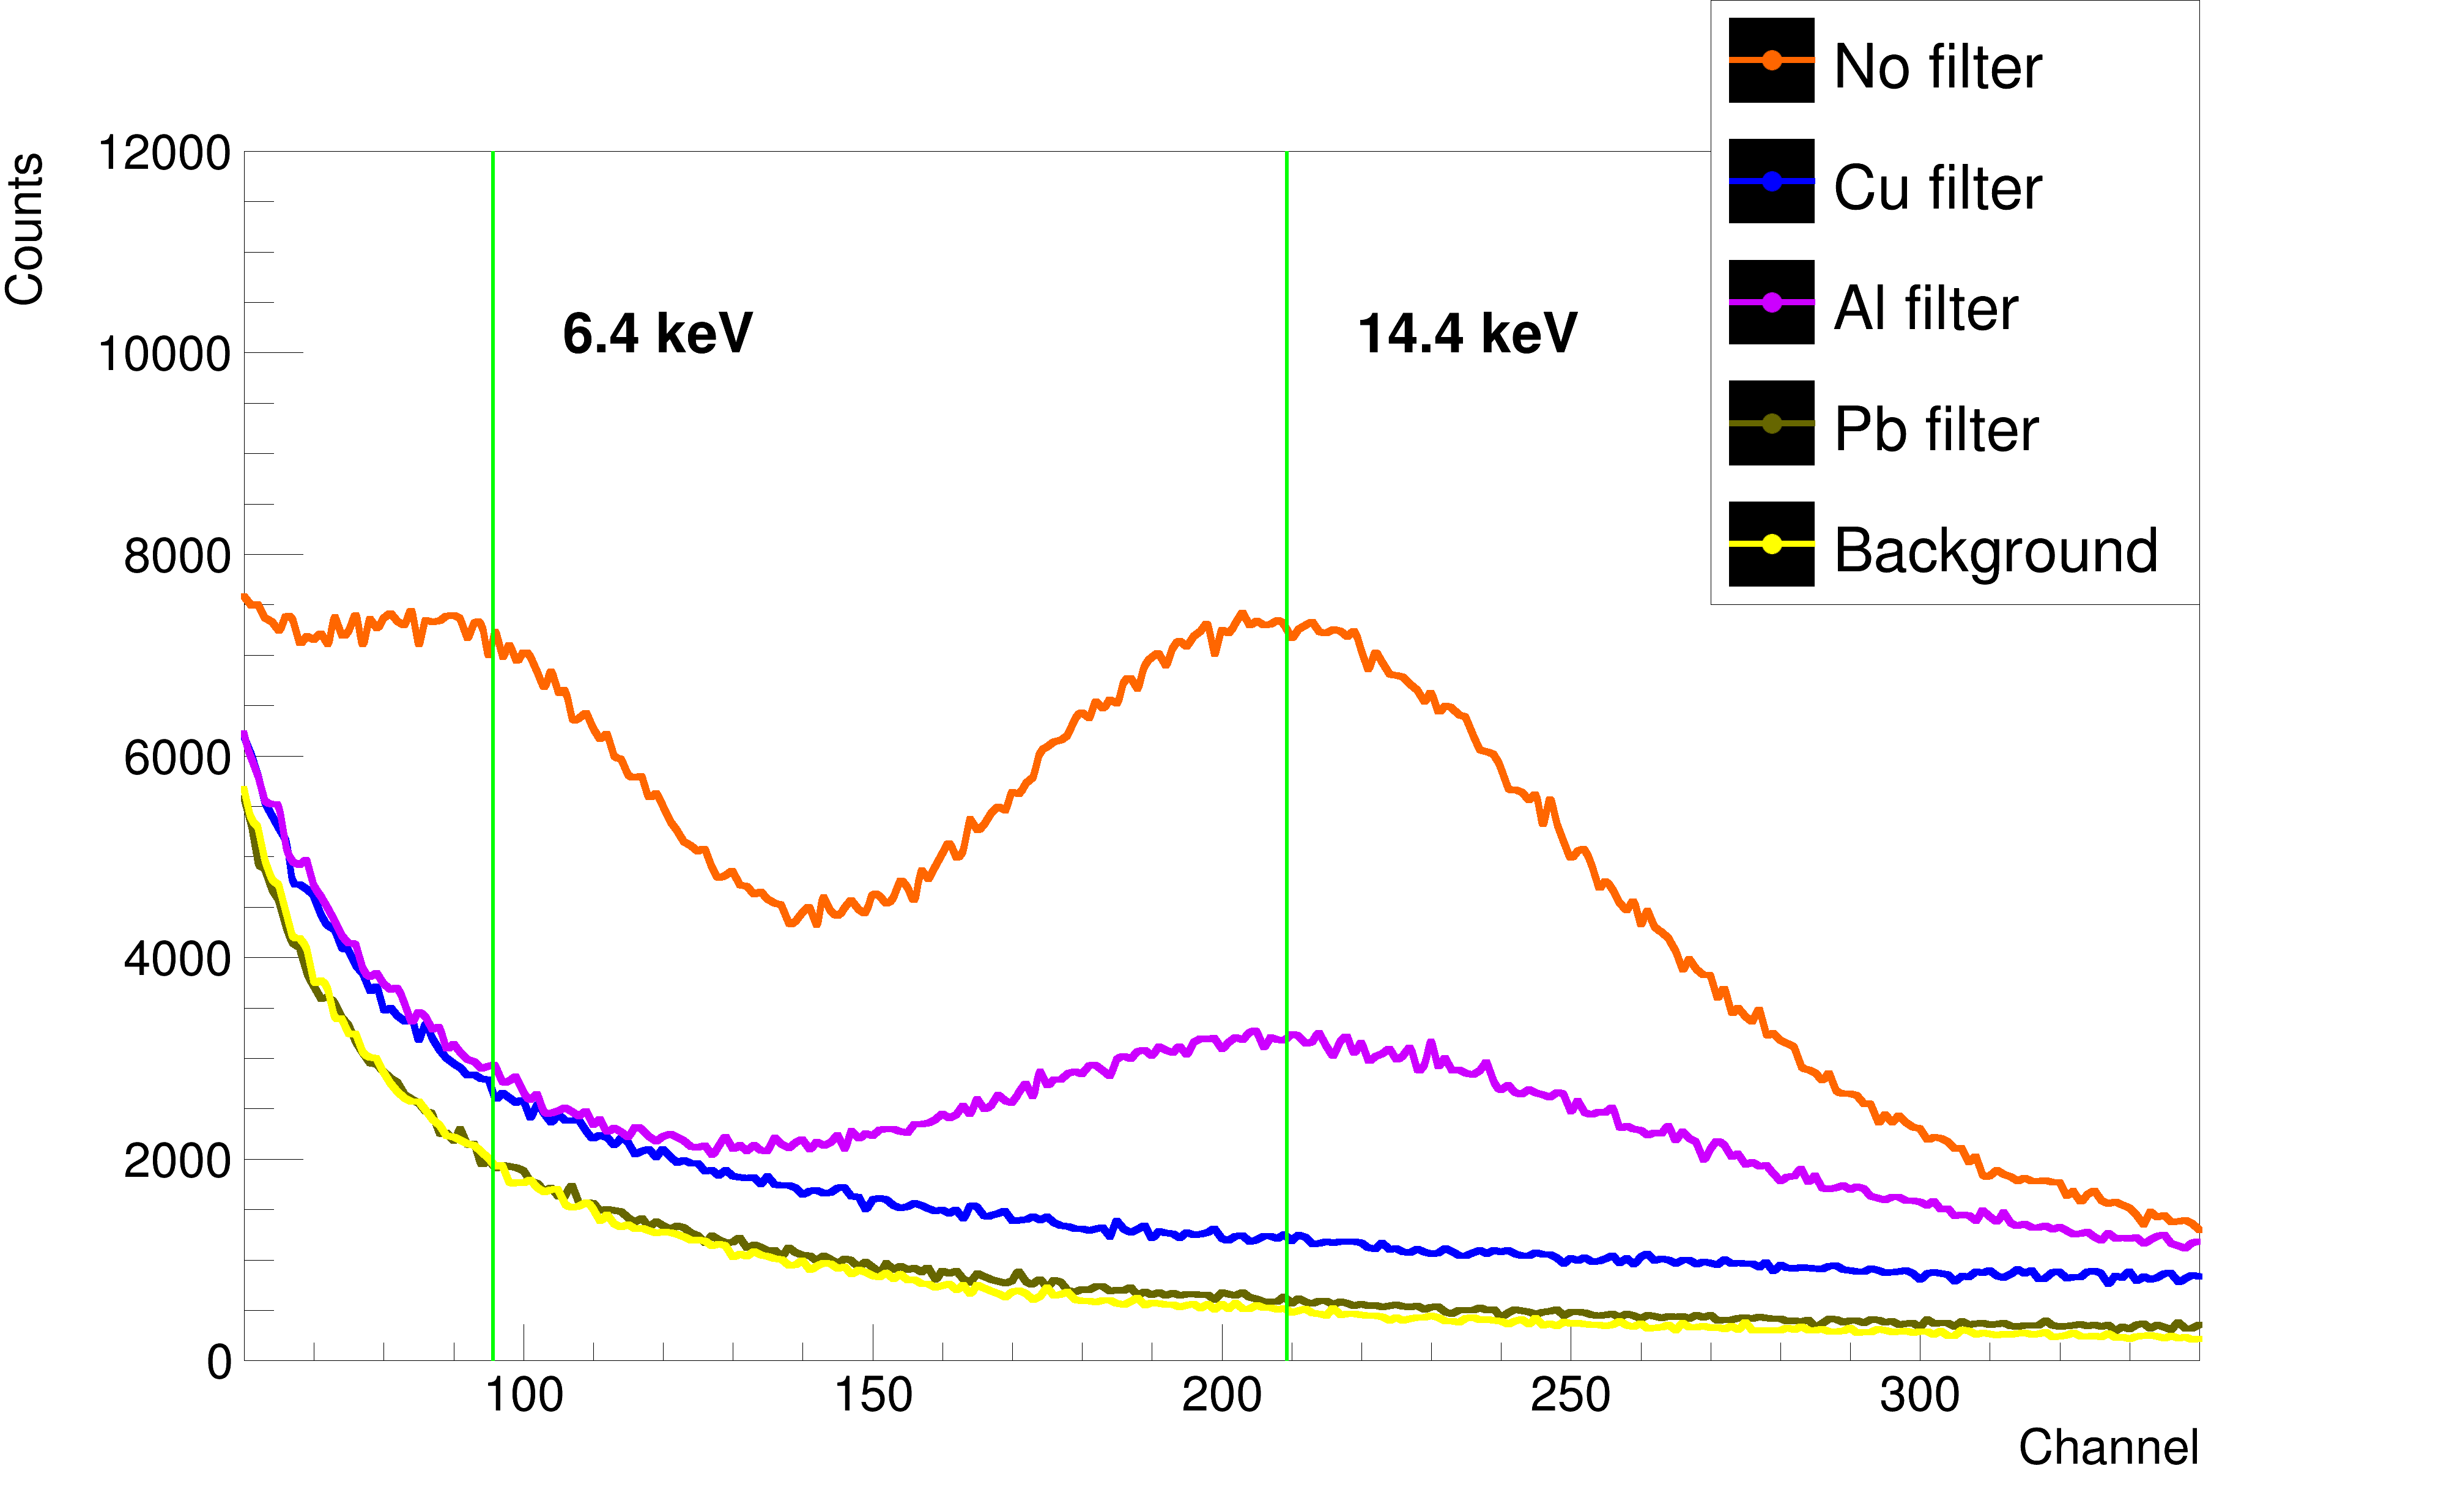
\includegraphics[scale=0.125, angle = 0]{./pictures/PMTSpectre.png}
\caption{Scintillator $^{57}$Co spectra.}
\label{Scintillator detector spectra.}
\end{figure}

\begin{figure}[H]
\centering
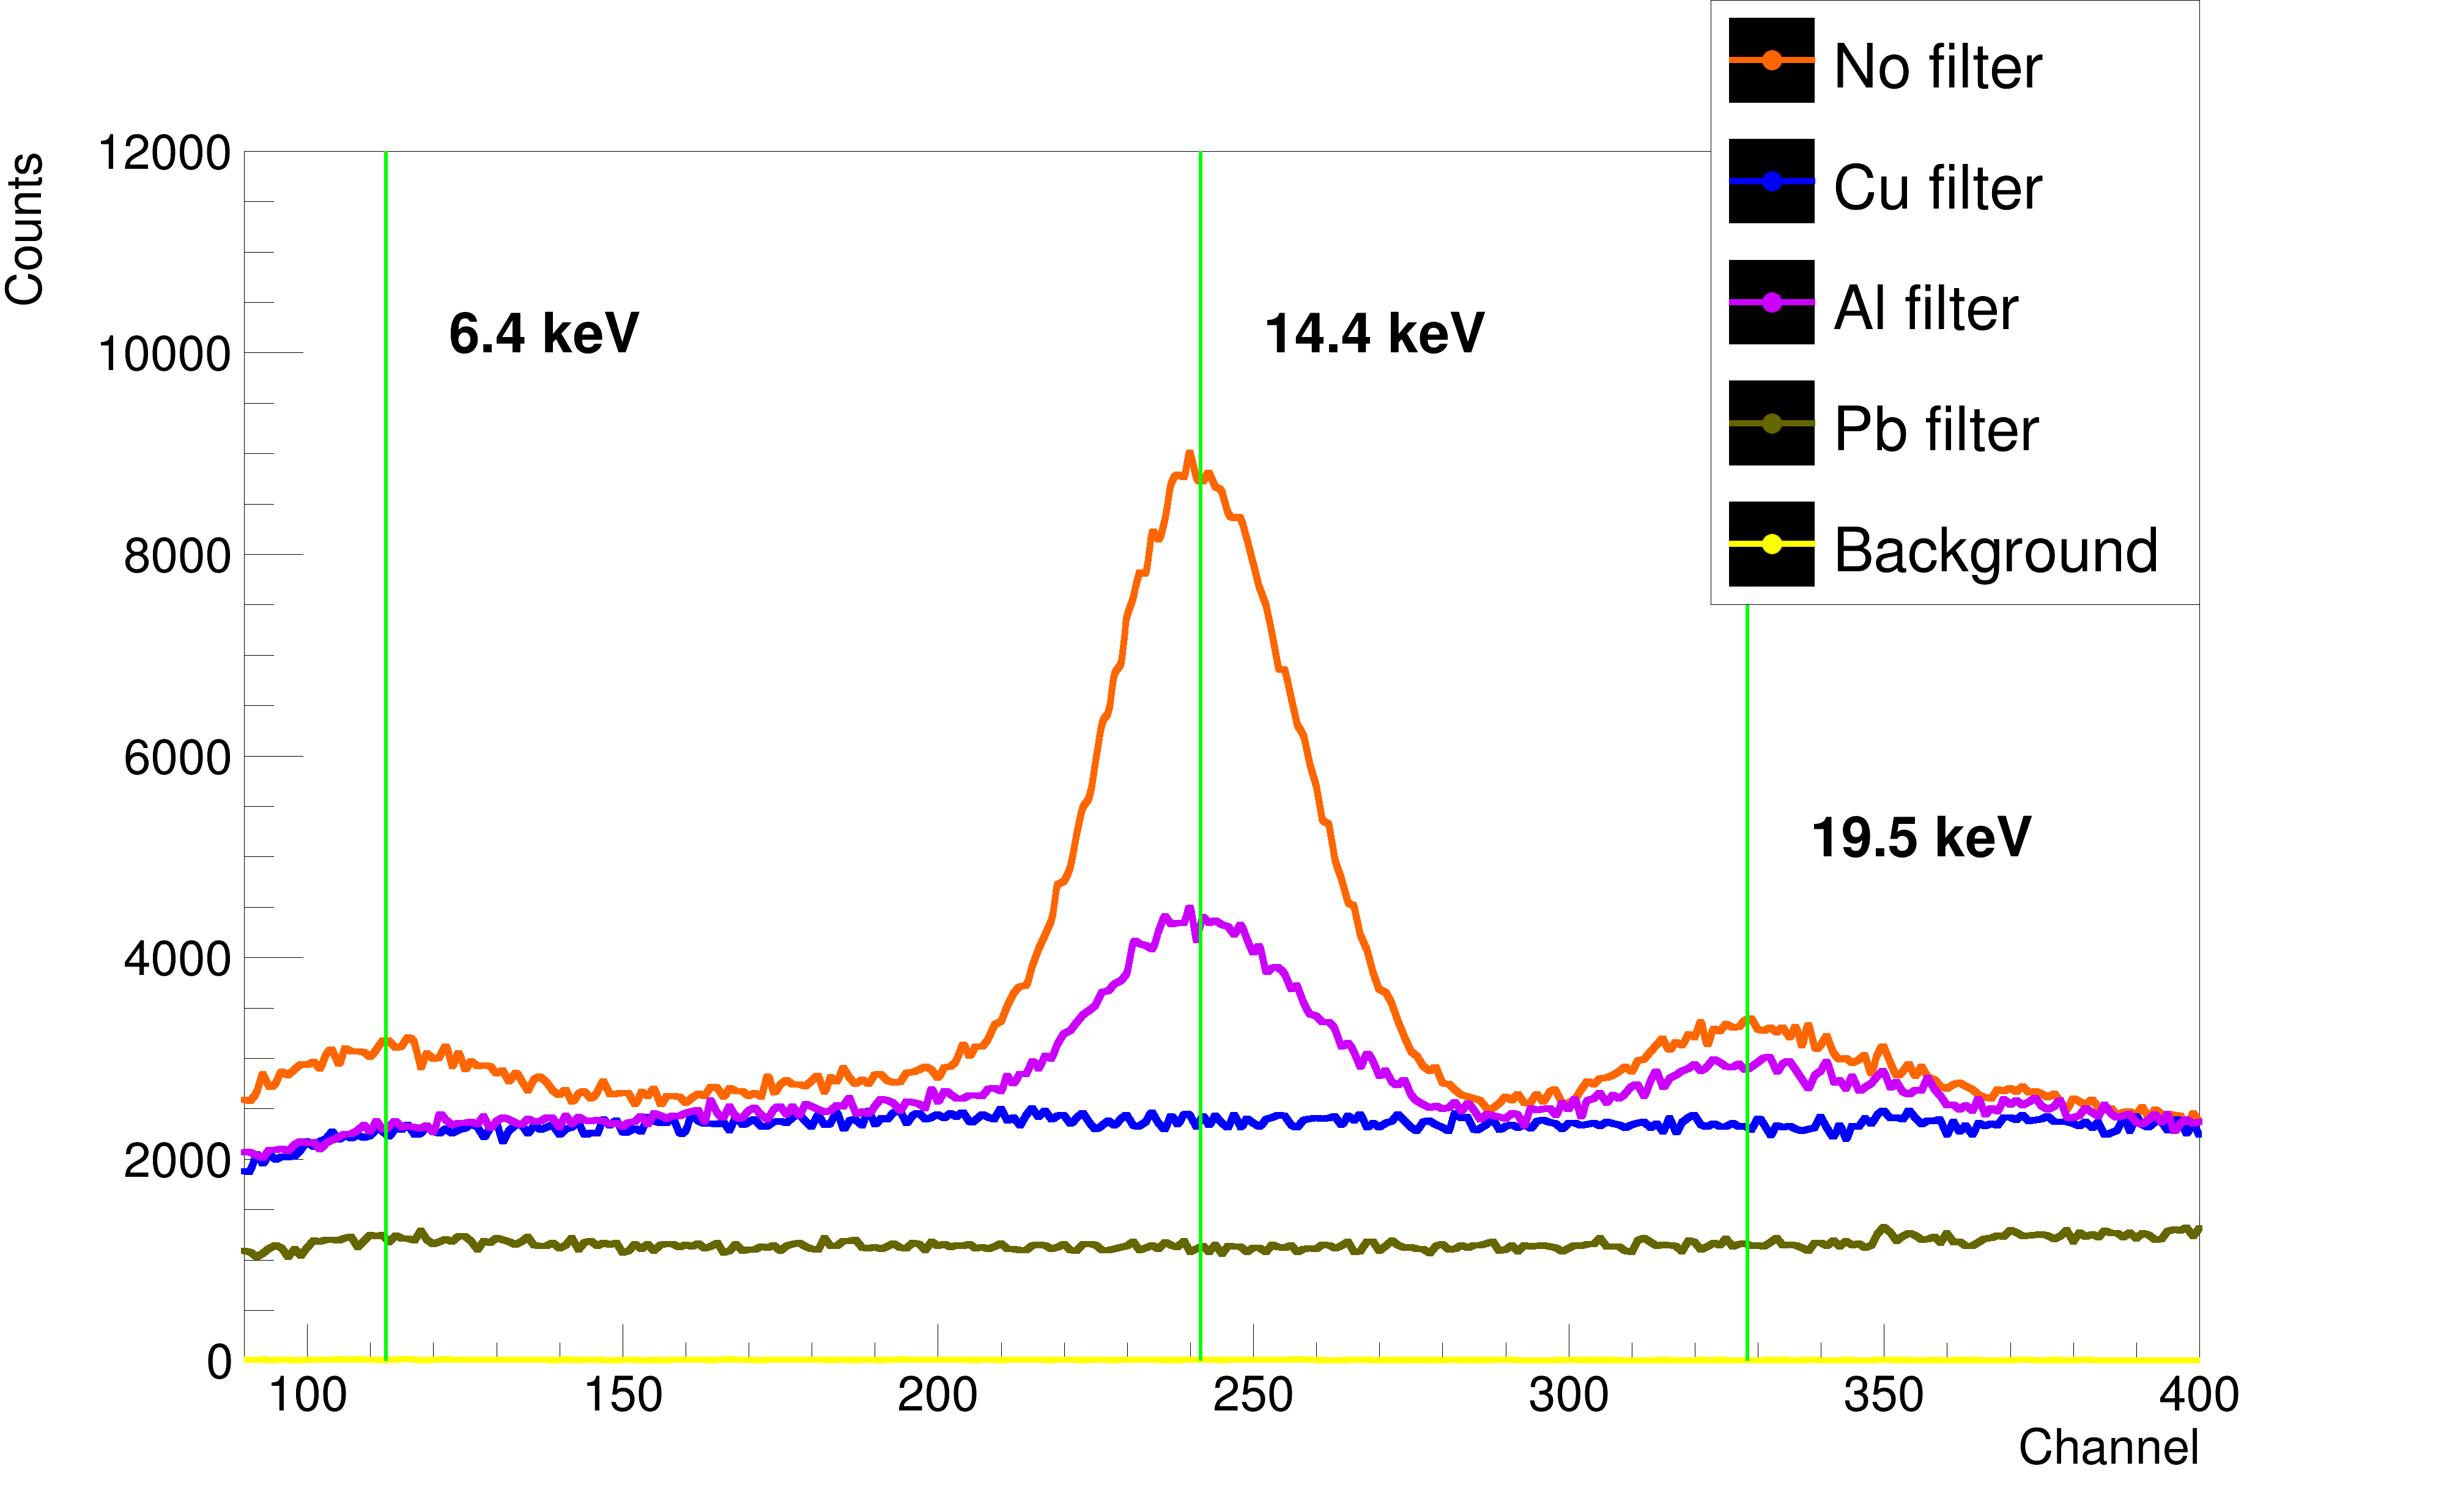
\includegraphics[scale=0.125, angle = 0]{./pictures/GasSpectre.png}
\caption{Gas $^{57}$Co spectra.}
\label{Gas detector spectra.}

\end{figure}


%In case of both detectors, both 14.4 keV and 6.4 keV peaks are fully observable. 
In spectra of gaseous detector, three narrow peaks can be observed - 14.4 keV peak and two small peaks - 6.4 keV and 19.5 keV. It also has a high level of Compton continuum.
The scintillator sees both 6.4 keV and 14.4 keV full energy peaks. However, its energy resolution is much worse - both peaks are noticeably wider and they overlap each other. 

\section{Results}
The sum of total counts for 14.4 keV and 6.4 keV full energy peaks along with the relative detection efficiency with respect to the most effective detector was calculated in the following way:

\begin{enumerate}
\item From the spectra without filter is subtracted the spectra with Cu filter. This provides a sufficient elimination of Compton continuum caused by 122 keV photons. 
\item The spectra obtained in previous step is fitted by a sum of Gaussians. Spectra of Si PIN and scintillator were fitted by sum of 2 Gaussians and in case of gas, the sum of 3 Gaussians is used.
\item The value of absolute counts (Gaussian's area) for the given energy spectra is calculated from the fit parameters with the uncertainties also taken from the fit.
\end{enumerate}




\begin{table}[H]
\centering
\begin{tabular}{|c|c|c|}
\hline
   & absolute & relative \\ \hline
Si PIN & $143000 \pm 3000$    & $0.291 \pm 0.008$  \\ \hline
gas & $231000 \pm 2000$    & $0.48 \pm  0.01$ \\ \hline
scintillator  & $491000 \pm 9000$    & $1$ \\ \hline
\end{tabular}
\caption{Table of calculated absolute and relative counts of 14.4 keV photons for each detector.}
 \label{144kevEFF}
\end{table}


The peak of 6.4 keV photons is not fully observable in the case of Si PIN detector. However, a rough estimation can be calculated using parameters obtained from Gaussian fit of partial 6.4 keV peak. Results in table \ref{64kevEFF} are considered to be only indicative. Note also that the setup wasn't designed to detect 6.4 keV photons - some detectors have slices of Al coating in detector window (Si PIN - ,scintillator - ,gas - window made of unknown metal).  

\begin{table}[H]
\centering
\begin{tabular}{|c|c|c|}
\hline
   & absolute & relative \\ \hline
Si PIN & $273000 \pm 8000$    & $1$  \\ \hline
gas & $20000 \pm 4000$    & $0.07 \pm 0.02$ \\ \hline
scintillator  & $184000 \pm 5000$    & $0.68 \pm 0.03$ \\ \hline
\end{tabular}
\caption{Table of calculated absolute and relative counts of 6.4 keV photons for each detector.}
 \label{64kevEFF}
\end{table}


\par
The results in table \ref{144kevEFF} show that the scintillator detector is the best detector for 14.4 keV photon among the three detectors that were tested. The Si PIN detector does not excel in detection of these energies and can be classified as the worst of the three. However, by the information provided by S14605 datasheet \cite{datS14605}, we come to a conclusion that the efficiency at 6.4 keV energies can be about 51 $\%$ better. This can be partially confirmed by rough estimations in table \ref{64kevEFF}, which describe the Si PIN as the best detector for 6.4 keV photons. To measure the full peak of 6.4 keV photons with S14605 photodiode, upgrades in electronics have to be made in order to increase the SNR, mainly the preamplifier has to be optimized for S14605's capacitance.



